% Options for packages loaded elsewhere
\PassOptionsToPackage{unicode}{hyperref}
\PassOptionsToPackage{hyphens}{url}
%
\documentclass[
]{article}
\title{Problem Set 1}
\author{Jingpeng Hong}
\date{Jan 24, 2022}

\usepackage{amsmath,amssymb}
\usepackage{lmodern}
\usepackage{iftex}
\ifPDFTeX
  \usepackage[T1]{fontenc}
  \usepackage[utf8]{inputenc}
  \usepackage{textcomp} % provide euro and other symbols
\else % if luatex or xetex
  \usepackage{unicode-math}
  \defaultfontfeatures{Scale=MatchLowercase}
  \defaultfontfeatures[\rmfamily]{Ligatures=TeX,Scale=1}
\fi
% Use upquote if available, for straight quotes in verbatim environments
\IfFileExists{upquote.sty}{\usepackage{upquote}}{}
\IfFileExists{microtype.sty}{% use microtype if available
  \usepackage[]{microtype}
  \UseMicrotypeSet[protrusion]{basicmath} % disable protrusion for tt fonts
}{}
\makeatletter
\@ifundefined{KOMAClassName}{% if non-KOMA class
  \IfFileExists{parskip.sty}{%
    \usepackage{parskip}
  }{% else
    \setlength{\parindent}{0pt}
    \setlength{\parskip}{6pt plus 2pt minus 1pt}}
}{% if KOMA class
  \KOMAoptions{parskip=half}}
\makeatother
\usepackage{xcolor}
\IfFileExists{xurl.sty}{\usepackage{xurl}}{} % add URL line breaks if available
\IfFileExists{bookmark.sty}{\usepackage{bookmark}}{\usepackage{hyperref}}
\hypersetup{
  pdftitle={Problem Set 1},
  pdfauthor={Jingpeng Hong},
  hidelinks,
  pdfcreator={LaTeX via pandoc}}
\urlstyle{same} % disable monospaced font for URLs
\usepackage[margin=1in]{geometry}
\usepackage{color}
\usepackage{fancyvrb}
\newcommand{\VerbBar}{|}
\newcommand{\VERB}{\Verb[commandchars=\\\{\}]}
\DefineVerbatimEnvironment{Highlighting}{Verbatim}{commandchars=\\\{\}}
% Add ',fontsize=\small' for more characters per line
\usepackage{framed}
\definecolor{shadecolor}{RGB}{248,248,248}
\newenvironment{Shaded}{\begin{snugshade}}{\end{snugshade}}
\newcommand{\AlertTok}[1]{\textcolor[rgb]{0.94,0.16,0.16}{#1}}
\newcommand{\AnnotationTok}[1]{\textcolor[rgb]{0.56,0.35,0.01}{\textbf{\textit{#1}}}}
\newcommand{\AttributeTok}[1]{\textcolor[rgb]{0.77,0.63,0.00}{#1}}
\newcommand{\BaseNTok}[1]{\textcolor[rgb]{0.00,0.00,0.81}{#1}}
\newcommand{\BuiltInTok}[1]{#1}
\newcommand{\CharTok}[1]{\textcolor[rgb]{0.31,0.60,0.02}{#1}}
\newcommand{\CommentTok}[1]{\textcolor[rgb]{0.56,0.35,0.01}{\textit{#1}}}
\newcommand{\CommentVarTok}[1]{\textcolor[rgb]{0.56,0.35,0.01}{\textbf{\textit{#1}}}}
\newcommand{\ConstantTok}[1]{\textcolor[rgb]{0.00,0.00,0.00}{#1}}
\newcommand{\ControlFlowTok}[1]{\textcolor[rgb]{0.13,0.29,0.53}{\textbf{#1}}}
\newcommand{\DataTypeTok}[1]{\textcolor[rgb]{0.13,0.29,0.53}{#1}}
\newcommand{\DecValTok}[1]{\textcolor[rgb]{0.00,0.00,0.81}{#1}}
\newcommand{\DocumentationTok}[1]{\textcolor[rgb]{0.56,0.35,0.01}{\textbf{\textit{#1}}}}
\newcommand{\ErrorTok}[1]{\textcolor[rgb]{0.64,0.00,0.00}{\textbf{#1}}}
\newcommand{\ExtensionTok}[1]{#1}
\newcommand{\FloatTok}[1]{\textcolor[rgb]{0.00,0.00,0.81}{#1}}
\newcommand{\FunctionTok}[1]{\textcolor[rgb]{0.00,0.00,0.00}{#1}}
\newcommand{\ImportTok}[1]{#1}
\newcommand{\InformationTok}[1]{\textcolor[rgb]{0.56,0.35,0.01}{\textbf{\textit{#1}}}}
\newcommand{\KeywordTok}[1]{\textcolor[rgb]{0.13,0.29,0.53}{\textbf{#1}}}
\newcommand{\NormalTok}[1]{#1}
\newcommand{\OperatorTok}[1]{\textcolor[rgb]{0.81,0.36,0.00}{\textbf{#1}}}
\newcommand{\OtherTok}[1]{\textcolor[rgb]{0.56,0.35,0.01}{#1}}
\newcommand{\PreprocessorTok}[1]{\textcolor[rgb]{0.56,0.35,0.01}{\textit{#1}}}
\newcommand{\RegionMarkerTok}[1]{#1}
\newcommand{\SpecialCharTok}[1]{\textcolor[rgb]{0.00,0.00,0.00}{#1}}
\newcommand{\SpecialStringTok}[1]{\textcolor[rgb]{0.31,0.60,0.02}{#1}}
\newcommand{\StringTok}[1]{\textcolor[rgb]{0.31,0.60,0.02}{#1}}
\newcommand{\VariableTok}[1]{\textcolor[rgb]{0.00,0.00,0.00}{#1}}
\newcommand{\VerbatimStringTok}[1]{\textcolor[rgb]{0.31,0.60,0.02}{#1}}
\newcommand{\WarningTok}[1]{\textcolor[rgb]{0.56,0.35,0.01}{\textbf{\textit{#1}}}}
\usepackage{graphicx}
\makeatletter
\def\maxwidth{\ifdim\Gin@nat@width>\linewidth\linewidth\else\Gin@nat@width\fi}
\def\maxheight{\ifdim\Gin@nat@height>\textheight\textheight\else\Gin@nat@height\fi}
\makeatother
% Scale images if necessary, so that they will not overflow the page
% margins by default, and it is still possible to overwrite the defaults
% using explicit options in \includegraphics[width, height, ...]{}
\setkeys{Gin}{width=\maxwidth,height=\maxheight,keepaspectratio}
% Set default figure placement to htbp
\makeatletter
\def\fps@figure{htbp}
\makeatother
\setlength{\emergencystretch}{3em} % prevent overfull lines
\providecommand{\tightlist}{%
  \setlength{\itemsep}{0pt}\setlength{\parskip}{0pt}}
\setcounter{secnumdepth}{-\maxdimen} % remove section numbering
\ifLuaTeX
  \usepackage{selnolig}  % disable illegal ligatures
\fi

\begin{document}
\maketitle

\hypertarget{question-1}{%
\subsection{Question 1}\label{question-1}}

\textbf{1.a.}

With the Bonferroni correction, we will reject the null when p-value is
less than \((1-\alpha)/p\). Hence the probability of false rejection of
the joint null is: \[P=1-(1-(1-\alpha)/p)^p\] Given the
\(\alpha = 0.95\)

\begin{Shaded}
\begin{Highlighting}[]
\NormalTok{p1}\OtherTok{=}\FunctionTok{seq}\NormalTok{(}\DecValTok{1}\NormalTok{, }\DecValTok{10}\NormalTok{, }\AttributeTok{by=}\DecValTok{1}\NormalTok{)}
\FunctionTok{plot}\NormalTok{(p1, }\DecValTok{1}\SpecialCharTok{{-}}\NormalTok{(}\DecValTok{1}\SpecialCharTok{{-}}\NormalTok{(}\DecValTok{1}\FloatTok{{-}0.95}\NormalTok{)}\SpecialCharTok{/}\NormalTok{p1)}\SpecialCharTok{**}\NormalTok{p1,}
\AttributeTok{main=}\StringTok{"Probability of false rejection versus p (0.95, Bonferroni correction)"}\NormalTok{, }\AttributeTok{ylab=}\StringTok{"Type I Error"}\NormalTok{, }\AttributeTok{xlab=}\StringTok{"p"}\NormalTok{, }\AttributeTok{type=}\StringTok{"l"}\NormalTok{, }\AttributeTok{col=}\StringTok{"blue"}\NormalTok{)}
\end{Highlighting}
\end{Shaded}

\includegraphics{PSet1_files/figure-latex/q1.a-1.pdf}

\textbf{1.b.}

\begin{Shaded}
\begin{Highlighting}[]
\NormalTok{N}\OtherTok{=}\DecValTok{20000}
\NormalTok{rho\_ls}\OtherTok{=}\FunctionTok{seq}\NormalTok{(}\DecValTok{0}\NormalTok{, }\DecValTok{1}\NormalTok{, }\AttributeTok{by=}\FloatTok{0.2}\NormalTok{)}
\NormalTok{p\_ls}\OtherTok{=}\FunctionTok{seq}\NormalTok{(}\DecValTok{1}\NormalTok{, }\DecValTok{10}\NormalTok{, }\AttributeTok{by=}\DecValTok{1}\NormalTok{)}
\NormalTok{prob\_error}\OtherTok{=}\FunctionTok{matrix}\NormalTok{(}\ConstantTok{NA}\NormalTok{, }\AttributeTok{nrow =} \FunctionTok{length}\NormalTok{(rho\_ls), }\AttributeTok{ncol =} \FunctionTok{length}\NormalTok{(p\_ls))}
\NormalTok{i}\OtherTok{=}\DecValTok{1}
\ControlFlowTok{for}\NormalTok{ (rho }\ControlFlowTok{in}\NormalTok{ rho\_ls) \{}
\NormalTok{  j}\OtherTok{=}\DecValTok{1}
  \ControlFlowTok{for}\NormalTok{ (p }\ControlFlowTok{in}\NormalTok{ p\_ls)\{}
\NormalTok{    covmat}\OtherTok{=}\FunctionTok{matrix}\NormalTok{(}\FunctionTok{rep}\NormalTok{(rho, p}\SpecialCharTok{*}\NormalTok{p), }\AttributeTok{nrow=}\NormalTok{p, }\AttributeTok{byrow=}\ConstantTok{TRUE}\NormalTok{)}
    \FunctionTok{diag}\NormalTok{(covmat)}\OtherTok{=}\DecValTok{1}
\NormalTok{    z}\OtherTok{=}\FunctionTok{mvrnorm}\NormalTok{(}\AttributeTok{n=}\NormalTok{N, }\AttributeTok{mu=}\FunctionTok{rep}\NormalTok{(}\DecValTok{0}\NormalTok{, p), }\AttributeTok{Sigma=}\NormalTok{covmat)}
\NormalTok{    c\_value}\OtherTok{=}\FunctionTok{qnorm}\NormalTok{(}\FloatTok{0.05}\SpecialCharTok{/}\NormalTok{p,}\AttributeTok{lower.tail =} \ConstantTok{FALSE}\NormalTok{)}
\NormalTok{    rej}\OtherTok{=}\NormalTok{z}\SpecialCharTok{\textgreater{}}\NormalTok{c\_value}
\NormalTok{    rejcol}\OtherTok{=}\NormalTok{(}\FunctionTok{rowSums}\NormalTok{(rej)}\SpecialCharTok{==}\DecValTok{0}\NormalTok{)}
\NormalTok{    prob\_error[i,j]}\OtherTok{=}\DecValTok{1}\SpecialCharTok{{-}}\FunctionTok{sum}\NormalTok{(rejcol)}\SpecialCharTok{/}\NormalTok{N}
\NormalTok{    j}\OtherTok{=}\NormalTok{j}\SpecialCharTok{+}\DecValTok{1}
\NormalTok{  \}}
\NormalTok{  i}\OtherTok{=}\NormalTok{i}\SpecialCharTok{+}\DecValTok{1}
\NormalTok{\}}
\FunctionTok{plot}\NormalTok{(p1, }\DecValTok{1}\SpecialCharTok{{-}}\NormalTok{(}\DecValTok{1}\SpecialCharTok{{-}}\NormalTok{(}\DecValTok{1}\FloatTok{{-}0.95}\NormalTok{)}\SpecialCharTok{/}\NormalTok{p1)}\SpecialCharTok{**}\NormalTok{p1, }\AttributeTok{main=}\StringTok{"Probability of false rejection versus p"}\NormalTok{, }\AttributeTok{ylab=}\StringTok{"Type I Error"}\NormalTok{, }\AttributeTok{type=}\StringTok{"l"}\NormalTok{, }\AttributeTok{xlab=}\StringTok{"p"}\NormalTok{, }\AttributeTok{ylim=}\FunctionTok{c}\NormalTok{(}\FloatTok{0.02}\NormalTok{,}\FloatTok{0.05}\NormalTok{), }\AttributeTok{col=}\StringTok{"blue"}\NormalTok{)}
\FunctionTok{lines}\NormalTok{(prob\_error[}\DecValTok{2}\NormalTok{,],}\AttributeTok{type=}\StringTok{"l"}\NormalTok{,}\AttributeTok{col=}\StringTok{"red"}\NormalTok{)}
\FunctionTok{lines}\NormalTok{(prob\_error[}\DecValTok{3}\NormalTok{,],}\AttributeTok{type=}\StringTok{"l"}\NormalTok{,}\AttributeTok{col=}\StringTok{"purple"}\NormalTok{)}
\FunctionTok{lines}\NormalTok{(prob\_error[}\DecValTok{4}\NormalTok{,],}\AttributeTok{type=}\StringTok{"l"}\NormalTok{,}\AttributeTok{col=}\StringTok{"green"}\NormalTok{)}
\FunctionTok{lines}\NormalTok{(prob\_error[}\DecValTok{5}\NormalTok{,],}\AttributeTok{type=}\StringTok{"l"}\NormalTok{,}\AttributeTok{col=}\StringTok{"orange"}\NormalTok{)}
\FunctionTok{legend}\NormalTok{(}\StringTok{"bottomleft"}\NormalTok{,}\AttributeTok{legend=}\FunctionTok{c}\NormalTok{(}\StringTok{"1.a"}\NormalTok{, }\StringTok{"rho=0.2"}\NormalTok{,}\StringTok{"rho=0.4"}\NormalTok{,}\StringTok{"rho=0.6"}\NormalTok{,}\StringTok{"rho=0.8"}\NormalTok{,}\StringTok{"rho=1.0"}\NormalTok{),}
       \AttributeTok{col=}\FunctionTok{c}\NormalTok{(}\StringTok{"blue"}\NormalTok{,}\StringTok{"red"}\NormalTok{,}\StringTok{"purple"}\NormalTok{,}\StringTok{"green"}\NormalTok{,}\StringTok{"orange"}\NormalTok{,}\StringTok{"black"}\NormalTok{), }\AttributeTok{lty=}\DecValTok{1}\NormalTok{,}\AttributeTok{lwd=}\DecValTok{2}\NormalTok{)}
\end{Highlighting}
\end{Shaded}

\includegraphics{PSet1_files/figure-latex/q1.b-1.pdf}

\textbf{1.c.}

The biggest value of \(\rho\) is 1, because the non-diagonal entries
denote the covariance. Given the variance of all \(z\) is 1 and the
correlation should lie between -1 and 1, the covariance should not be
greater than 1.

\hypertarget{question-2}{%
\subsection{Question 2}\label{question-2}}

\textbf{2.a. Download the data set Hitters from the ISLR library.}

\begin{Shaded}
\begin{Highlighting}[]
\FunctionTok{library}\NormalTok{(ISLR)}
\end{Highlighting}
\end{Shaded}

\textbf{2.b. Divide the dataset into a training set and a test set.}

The trade off between having a big training/small test versus small
training/big test:

\begin{enumerate}
\def\labelenumi{\arabic{enumi})}
\item
  If we have a big training, there will be fewer observations for us to
  estimate the test error rate. Hence, the validation set error rate
  will have big variance and lead to a poor estimate of the test error
  rate. In other words, we cannot know the out-of-sample prediction
  power of the model well.
\item
  If we have a small training, we cannot have enough observations to
  train the model. In this way, our estimation of parameters will have
  greater variance.
\end{enumerate}

I choose 70\% training and 30\% test. I use most of the data to train,
but will still have sufficient data for out-of-sample evaluation.

\begin{Shaded}
\begin{Highlighting}[]
\NormalTok{Hitters}\OtherTok{=}\FunctionTok{na.omit}\NormalTok{(Hitters) }\CommentTok{\# omit the observations with missing values}
\FunctionTok{set.seed}\NormalTok{(}\DecValTok{1}\NormalTok{)}
\NormalTok{train}\OtherTok{=}\FunctionTok{sample}\NormalTok{(}\FunctionTok{c}\NormalTok{(}\ConstantTok{TRUE}\NormalTok{,}\ConstantTok{FALSE}\NormalTok{), }\AttributeTok{size=}\FunctionTok{nrow}\NormalTok{(Hitters), }\AttributeTok{rep=}\ConstantTok{TRUE}\NormalTok{, }\AttributeTok{prob=}\FunctionTok{c}\NormalTok{(}\FloatTok{0.7}\NormalTok{,}\FloatTok{0.3}\NormalTok{)) }\CommentTok{\# train/test=7/3}
\NormalTok{test}\OtherTok{=}\NormalTok{(}\SpecialCharTok{!}\NormalTok{train)}
\end{Highlighting}
\end{Shaded}

\textbf{2.c. Select the model made of the 7 coefficients.}

The model made of the 7 coefficients with the smallest p-values is
\texttt{PutOuts}, \texttt{Walks}, \texttt{CHits}, \texttt{CAtBat},
\texttt{DivisionW}, \texttt{AtBat} and \texttt{Hits}

\begin{Shaded}
\begin{Highlighting}[]
\NormalTok{reg.train}\OtherTok{=}\FunctionTok{glm}\NormalTok{(Salary}\SpecialCharTok{\textasciitilde{}}\NormalTok{., }\AttributeTok{data=}\NormalTok{Hitters[train,])}
\NormalTok{pvalue}\OtherTok{=}\FunctionTok{coef}\NormalTok{(}\FunctionTok{summary}\NormalTok{(reg.train))[, }\DecValTok{4}\NormalTok{]}
\NormalTok{pvalue}\OtherTok{=}\FunctionTok{sort}\NormalTok{(pvalue, }\AttributeTok{decreasing=}\ConstantTok{FALSE}\NormalTok{)}
\end{Highlighting}
\end{Shaded}

\textbf{2.d. Select the best model made of 7 coefficients according to
the forward stepwise selection procedure.}

Forward stepwise selection procedure: Suppose there are \(p\)
predictors. We begin with a model containing no predictors, and then add
one predictors each time until all of the predictors are in the model.
In particular, at each step we choose the best variable that gives the
greatest additional improvement to the fit. Finally, we select a single
best model from the \(p+1\) models.

The best model here is \texttt{CRuns}, \texttt{Hits}, \texttt{PutOuts},
\texttt{AtBat}, \texttt{RBI}, \texttt{CWalks} and \texttt{Walks}

In c, we select the most significant variable from the full model at the
same time. However, in forward stepwise selection procedure, we start
with the most significant variable, and add the most significant one
among the rest. The forward stepwise selection procedure will be less
sensitive to the correlation among variables (e.g.~collinearity).

\begin{Shaded}
\begin{Highlighting}[]
\NormalTok{regfit.train.fwd}\OtherTok{=}\FunctionTok{regsubsets}\NormalTok{(Salary}\SpecialCharTok{\textasciitilde{}}\NormalTok{.,}\AttributeTok{data=}\NormalTok{Hitters[train,], }\AttributeTok{nvmax=}\DecValTok{7}\NormalTok{, }\AttributeTok{method=}\StringTok{"forward"}\NormalTok{)}
\FunctionTok{summary}\NormalTok{(regfit.train.fwd)}
\end{Highlighting}
\end{Shaded}

\begin{verbatim}
## Subset selection object
## Call: regsubsets.formula(Salary ~ ., data = Hitters[train, ], nvmax = 7, 
##     method = "forward")
## 19 Variables  (and intercept)
##            Forced in Forced out
## AtBat          FALSE      FALSE
## Hits           FALSE      FALSE
## HmRun          FALSE      FALSE
## Runs           FALSE      FALSE
## RBI            FALSE      FALSE
## Walks          FALSE      FALSE
## Years          FALSE      FALSE
## CAtBat         FALSE      FALSE
## CHits          FALSE      FALSE
## CHmRun         FALSE      FALSE
## CRuns          FALSE      FALSE
## CRBI           FALSE      FALSE
## CWalks         FALSE      FALSE
## LeagueN        FALSE      FALSE
## DivisionW      FALSE      FALSE
## PutOuts        FALSE      FALSE
## Assists        FALSE      FALSE
## Errors         FALSE      FALSE
## NewLeagueN     FALSE      FALSE
## 1 subsets of each size up to 7
## Selection Algorithm: forward
##          AtBat Hits HmRun Runs RBI Walks Years CAtBat CHits CHmRun CRuns CRBI
## 1  ( 1 ) " "   " "  " "   " "  " " " "   " "   " "    " "   " "    "*"   " " 
## 2  ( 1 ) " "   "*"  " "   " "  " " " "   " "   " "    " "   " "    "*"   " " 
## 3  ( 1 ) " "   "*"  " "   " "  " " " "   " "   " "    " "   " "    "*"   " " 
## 4  ( 1 ) "*"   "*"  " "   " "  " " " "   " "   " "    " "   " "    "*"   " " 
## 5  ( 1 ) "*"   "*"  " "   " "  "*" " "   " "   " "    " "   " "    "*"   " " 
## 6  ( 1 ) "*"   "*"  " "   " "  "*" " "   " "   " "    " "   " "    "*"   " " 
## 7  ( 1 ) "*"   "*"  " "   " "  "*" "*"   " "   " "    " "   " "    "*"   " " 
##          CWalks LeagueN DivisionW PutOuts Assists Errors NewLeagueN
## 1  ( 1 ) " "    " "     " "       " "     " "     " "    " "       
## 2  ( 1 ) " "    " "     " "       " "     " "     " "    " "       
## 3  ( 1 ) " "    " "     " "       "*"     " "     " "    " "       
## 4  ( 1 ) " "    " "     " "       "*"     " "     " "    " "       
## 5  ( 1 ) " "    " "     " "       "*"     " "     " "    " "       
## 6  ( 1 ) "*"    " "     " "       "*"     " "     " "    " "       
## 7  ( 1 ) "*"    " "     " "       "*"     " "     " "    " "
\end{verbatim}

\textbf{2.e. Select the best model made of 7 coefficients according to
the best subset procedure.}

\begin{Shaded}
\begin{Highlighting}[]
\NormalTok{regfit.train}\OtherTok{=}\FunctionTok{regsubsets}\NormalTok{(Salary}\SpecialCharTok{\textasciitilde{}}\NormalTok{.,}\AttributeTok{data=}\NormalTok{Hitters[train,], }\AttributeTok{nvmax=}\DecValTok{7}\NormalTok{)}
\FunctionTok{summary}\NormalTok{(regfit.train)}
\end{Highlighting}
\end{Shaded}

\begin{verbatim}
## Subset selection object
## Call: regsubsets.formula(Salary ~ ., data = Hitters[train, ], nvmax = 7)
## 19 Variables  (and intercept)
##            Forced in Forced out
## AtBat          FALSE      FALSE
## Hits           FALSE      FALSE
## HmRun          FALSE      FALSE
## Runs           FALSE      FALSE
## RBI            FALSE      FALSE
## Walks          FALSE      FALSE
## Years          FALSE      FALSE
## CAtBat         FALSE      FALSE
## CHits          FALSE      FALSE
## CHmRun         FALSE      FALSE
## CRuns          FALSE      FALSE
## CRBI           FALSE      FALSE
## CWalks         FALSE      FALSE
## LeagueN        FALSE      FALSE
## DivisionW      FALSE      FALSE
## PutOuts        FALSE      FALSE
## Assists        FALSE      FALSE
## Errors         FALSE      FALSE
## NewLeagueN     FALSE      FALSE
## 1 subsets of each size up to 7
## Selection Algorithm: exhaustive
##          AtBat Hits HmRun Runs RBI Walks Years CAtBat CHits CHmRun CRuns CRBI
## 1  ( 1 ) " "   " "  " "   " "  " " " "   " "   " "    " "   " "    "*"   " " 
## 2  ( 1 ) " "   "*"  " "   " "  " " " "   " "   " "    " "   " "    " "   "*" 
## 3  ( 1 ) " "   " "  " "   " "  "*" " "   " "   "*"    "*"   " "    " "   " " 
## 4  ( 1 ) " "   " "  " "   "*"  " " " "   " "   "*"    "*"   " "    " "   " " 
## 5  ( 1 ) " "   " "  " "   " "  "*" "*"   " "   "*"    "*"   " "    " "   " " 
## 6  ( 1 ) " "   " "  " "   " "  "*" "*"   " "   "*"    "*"   " "    " "   " " 
## 7  ( 1 ) " "   "*"  " "   " "  " " "*"   " "   "*"    "*"   "*"    " "   " " 
##          CWalks LeagueN DivisionW PutOuts Assists Errors NewLeagueN
## 1  ( 1 ) " "    " "     " "       " "     " "     " "    " "       
## 2  ( 1 ) " "    " "     " "       " "     " "     " "    " "       
## 3  ( 1 ) " "    " "     " "       " "     " "     " "    " "       
## 4  ( 1 ) " "    " "     " "       "*"     " "     " "    " "       
## 5  ( 1 ) " "    " "     " "       "*"     " "     " "    " "       
## 6  ( 1 ) " "    " "     "*"       "*"     " "     " "    " "       
## 7  ( 1 ) " "    " "     "*"       "*"     " "     " "    " "
\end{verbatim}

\textbf{2.f. Compute the sample mean squared error in the test set for
each method fitted in c, d and e, and collect the results in a table.}

~model \textbar{} MSE \textbar{}\\
c \textbar{} 490057322.8 \textbar{}\\
d \textbar{} 177373.1 \textbar{}\\
e \textbar{} 181767.2 \textbar{}

\begin{Shaded}
\begin{Highlighting}[]
\NormalTok{test.mat}\OtherTok{=}\FunctionTok{model.matrix}\NormalTok{(Salary}\SpecialCharTok{\textasciitilde{}}\NormalTok{.,}\AttributeTok{data=}\NormalTok{Hitters[test,])}
\NormalTok{mse.test}\OtherTok{=}\FunctionTok{rep}\NormalTok{(}\ConstantTok{NA}\NormalTok{,}\DecValTok{3}\NormalTok{)}
\CommentTok{\# MSE in c}
\NormalTok{coefc}\OtherTok{=}\FunctionTok{coef}\NormalTok{(}\FunctionTok{summary}\NormalTok{(reg.train))[}\FunctionTok{order}\NormalTok{(pvalue, }\AttributeTok{decreasing=}\ConstantTok{FALSE}\NormalTok{)][}\DecValTok{1}\SpecialCharTok{:}\DecValTok{7}\NormalTok{]}
\NormalTok{predc}\OtherTok{=}\NormalTok{test.mat[,}\FunctionTok{names}\NormalTok{(}\FunctionTok{sort}\NormalTok{(pvalue, }\AttributeTok{decreasing=}\ConstantTok{FALSE}\NormalTok{)[}\DecValTok{1}\SpecialCharTok{:}\DecValTok{7}\NormalTok{])]}\SpecialCharTok{\%*\%}\NormalTok{coefc}
\NormalTok{mse.test[}\DecValTok{1}\NormalTok{]}\OtherTok{=}\FunctionTok{mean}\NormalTok{((Hitters}\SpecialCharTok{$}\NormalTok{Salary[test]}\SpecialCharTok{{-}}\NormalTok{predc)}\SpecialCharTok{\^{}}\DecValTok{2}\NormalTok{)}
\CommentTok{\# MSE in d}
\NormalTok{coefd}\OtherTok{=}\FunctionTok{coef}\NormalTok{(regfit.train.fwd, }\AttributeTok{id=}\DecValTok{7}\NormalTok{)}
\NormalTok{predd}\OtherTok{=}\NormalTok{test.mat[,}\FunctionTok{names}\NormalTok{(coefd)]}\SpecialCharTok{\%*\%}\NormalTok{coefd}
\NormalTok{mse.test[}\DecValTok{2}\NormalTok{]}\OtherTok{=}\FunctionTok{mean}\NormalTok{((Hitters}\SpecialCharTok{$}\NormalTok{Salary[test]}\SpecialCharTok{{-}}\NormalTok{predd)}\SpecialCharTok{\^{}}\DecValTok{2}\NormalTok{)}
\CommentTok{\# MSE in e}
\NormalTok{coefe}\OtherTok{=}\FunctionTok{coef}\NormalTok{(regfit.train, }\AttributeTok{id=}\DecValTok{7}\NormalTok{)}
\NormalTok{prede}\OtherTok{=}\NormalTok{test.mat[,}\FunctionTok{names}\NormalTok{(coefe)]}\SpecialCharTok{\%*\%}\NormalTok{coefe}
\NormalTok{mse.test[}\DecValTok{3}\NormalTok{]}\OtherTok{=}\FunctionTok{mean}\NormalTok{((Hitters}\SpecialCharTok{$}\NormalTok{Salary[test]}\SpecialCharTok{{-}}\NormalTok{prede)}\SpecialCharTok{\^{}}\DecValTok{2}\NormalTok{)}
\NormalTok{mse.test}
\end{Highlighting}
\end{Shaded}

\begin{verbatim}
## [1] 490057322.8    177373.1    181767.2
\end{verbatim}

\textbf{2.g. Repeat exercises c-f for different sizes of the subset of
coefficients, and present your results in an extended table or plot.}

\hypertarget{question-3}{%
\subsection{Question 3}\label{question-3}}

\textbf{3.a.}

The in-sample sum-of-squared errors for this regression is
\texttt{726316624}and \(R^2\) is \texttt{0.734876}

\begin{Shaded}
\begin{Highlighting}[]
\NormalTok{biketab}\OtherTok{=}\FunctionTok{fread}\NormalTok{(}\StringTok{"bikeshare.csv"}\NormalTok{)}
\CommentTok{\# tell R which are factors}
\NormalTok{biketab[, }\FunctionTok{c}\NormalTok{(}\StringTok{"dteday"}\NormalTok{, }\StringTok{"mnth"}\NormalTok{,}\StringTok{"season"}\NormalTok{,}\StringTok{"weekday"}\NormalTok{,}\StringTok{"hr"}\NormalTok{,}\StringTok{"weathersit"}\NormalTok{) }\SpecialCharTok{:}\ErrorTok{=} \FunctionTok{list}\NormalTok{(}
  \FunctionTok{factor}\NormalTok{(dteday), }\FunctionTok{factor}\NormalTok{(mnth), }\FunctionTok{factor}\NormalTok{(season), }
  \FunctionTok{factor}\NormalTok{(weekday), }\FunctionTok{factor}\NormalTok{(hr), }\FunctionTok{factor}\NormalTok{(weathersit))] }
\CommentTok{\# calculates total cnt by day, also keeping track of the corresponding yr and mnth id.}
\NormalTok{daytots}\OtherTok{=}\NormalTok{biketab[, }\FunctionTok{list}\NormalTok{(}\AttributeTok{total=}\FunctionTok{sum}\NormalTok{(cnt)), by}\OtherTok{=}\FunctionTok{c}\NormalTok{(}\StringTok{"dteday"}\NormalTok{,}\StringTok{"yr"}\NormalTok{,}\StringTok{"mnth"}\NormalTok{)]}
\FunctionTok{row.names}\NormalTok{(daytots)}\OtherTok{=}\NormalTok{daytots}\SpecialCharTok{$}\NormalTok{dteday}
\CommentTok{\# simple regression}
\NormalTok{daylm}\OtherTok{=}\FunctionTok{glm}\NormalTok{(total }\SpecialCharTok{\textasciitilde{}}\NormalTok{ yr}\SpecialCharTok{*}\NormalTok{mnth, }\AttributeTok{data=}\NormalTok{daytots)}
\FunctionTok{names}\NormalTok{(daylm)}
\end{Highlighting}
\end{Shaded}

\begin{verbatim}
##  [1] "coefficients"      "residuals"         "fitted.values"    
##  [4] "effects"           "R"                 "rank"             
##  [7] "qr"                "family"            "linear.predictors"
## [10] "deviance"          "aic"               "null.deviance"    
## [13] "iter"              "weights"           "prior.weights"    
## [16] "df.residual"       "df.null"           "y"                
## [19] "converged"         "boundary"          "model"            
## [22] "call"              "formula"           "terms"            
## [25] "data"              "offset"            "control"          
## [28] "method"            "contrasts"         "xlevels"
\end{verbatim}

\begin{Shaded}
\begin{Highlighting}[]
\CommentTok{\# calculate in{-}sample sum{-}of{-}squared errors}
\NormalTok{sse}\OtherTok{=}\NormalTok{daylm}\SpecialCharTok{$}\NormalTok{deviance}
\FunctionTok{print}\NormalTok{(sse)}
\end{Highlighting}
\end{Shaded}

\begin{verbatim}
## [1] 726316624
\end{verbatim}

\begin{Shaded}
\begin{Highlighting}[]
\CommentTok{\# calculate R\^{}2}
\NormalTok{rsqr}\OtherTok{=}\DecValTok{1} \SpecialCharTok{{-}}\NormalTok{ daylm}\SpecialCharTok{$}\NormalTok{deviance}\SpecialCharTok{/}\NormalTok{daylm}\SpecialCharTok{$}\NormalTok{null.deviance}
\FunctionTok{print}\NormalTok{(rsqr)}
\end{Highlighting}
\end{Shaded}

\begin{verbatim}
## [1] 0.734876
\end{verbatim}

\textbf{3.b.}

The mathematical formula for \texttt{daylm} is
\[Total_i = \beta_0 + \beta_1 yr_i + \beta_2 mnth2_i+... + \beta_{12} mnth12_i+\beta_{1,2} yr_i \times mnth2_i+... + \beta_{1,12} yr_i \times mnth12_i+\epsilon_i\]
The assumption we have here is that:

\begin{enumerate}
\def\labelenumi{\arabic{enumi})}
\tightlist
\item
  \((Total_i, yr_i, mnth1_i,..., mnth12_i)\) is i.i.d.
\item
  \(E[\epsilon_i|X] = 0\)
\end{enumerate}

From the OLS, we minimize the function:
\[\sum(Total_i-X_i'\hat{\beta})^2\]

The criticism is that since this is a time-series data set, there will
be the correlation of error terms, which violates the i.i.d. assumption.

\textbf{3.c.}

The null hypothesis is that the standardized residuals are drawn from
the identical distribution \(N(0,1)\) independently. Small values
indicate the possibility that the data point is drawn from the
distribution \(N(0,1)\) is low. In other words, it have the different
distribution with other days, which indicates a possible outlier day.

\begin{Shaded}
\begin{Highlighting}[]
\NormalTok{rse}\OtherTok{=}\FunctionTok{sqrt}\NormalTok{(daylm}\SpecialCharTok{$}\NormalTok{deviance}\SpecialCharTok{/}\NormalTok{daylm}\SpecialCharTok{$}\NormalTok{df.residual) }\CommentTok{\# calculate residual standard error}
\NormalTok{std\_resids}\OtherTok{=}\NormalTok{(}\FunctionTok{fitted}\NormalTok{(daylm) }\SpecialCharTok{{-}}\NormalTok{ daytots}\SpecialCharTok{$}\NormalTok{total)}\SpecialCharTok{/}\NormalTok{rse }\CommentTok{\# standardization}
\NormalTok{pvalue}\OtherTok{=}\FunctionTok{pnorm}\NormalTok{(}\SpecialCharTok{{-}}\FunctionTok{abs}\NormalTok{(std\_resids)) }\CommentTok{\# calculate outlier p{-}values}
\end{Highlighting}
\end{Shaded}

\textbf{3.d. Plot the p-value distribution.}

The distribution of p-value is similar to a uniform distribution, which
indicates that the standardized residuals follow the \(N(0,1)\) and our
assumption that \(\epsilon ~ N(0,1)\) is likelt to hold.

\begin{Shaded}
\begin{Highlighting}[]
\FunctionTok{plot}\NormalTok{(}\FunctionTok{density}\NormalTok{(}\DecValTok{2}\SpecialCharTok{*}\NormalTok{pvalue))}
\end{Highlighting}
\end{Shaded}

\includegraphics{PSet1_files/figure-latex/q3.d-1.pdf}

\hypertarget{question-4}{%
\subsection{Question 4}\label{question-4}}

Consider the model with \(X_1\) and \(X_2\):
\[Y=X_1\hat{\beta_1}+X_2\hat{\beta_2}+\hat{\epsilon}\] Given the
projection matrix of \(X_1\): \[P_1=X_1(X_1^TX_1)^{-1}X_1^T\] Then we
have: \[P_1Y=P_1X_1\hat{\beta_1}+P_1X_2\hat{\beta_2}+P_1\hat{\epsilon}\]
Here, \(P_1Y\) is the light green line,
\(P_1X_1\hat{\beta_1}=X_1\hat{\beta_1}\) is the true effect (the red
line). \(P_1X_2\hat{\beta_2}\) is the projection of \(X_2\hat{\beta_2}\)
on the span of \(X_1\), which is the omitted variable bias here.
\(P_1\hat{\epsilon}=0\) by definition.

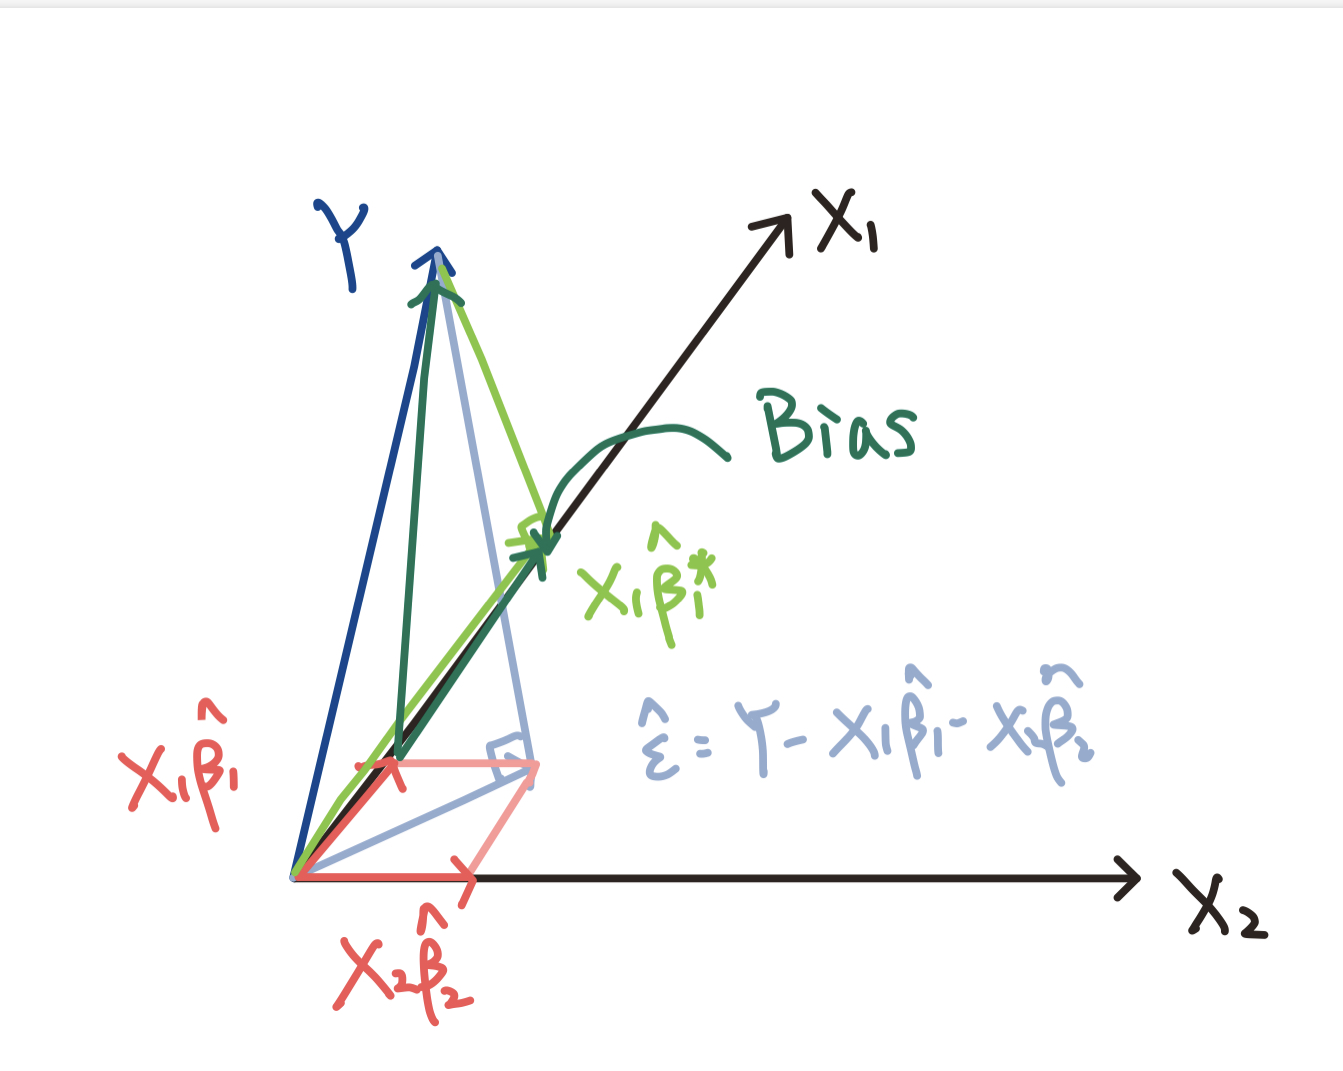
\includegraphics{graph_Q4.jpg}

\end{document}
